\documentclass[]{article}
%source: https://tex.stackexchange.com/questions/213860/how-to-generate-a-named-destination-in-pdf
\usepackage{blindtext}
\usepackage{hyperref}
\usepackage{graphicx}

\usepackage{bookmark}
\begin{document}

\newpage
\section{About this document}
\hypertarget{about_this_document}{}%
%defining the named destination "about_this_document
\blindtext[10]

\newpage
\section{Safety}
%defining the named destination "safety"
\hypertarget{safety}{}%
\blindtext[10]

\newpage
\section{Installation}
%defining the named destination "installation"
\hypertarget{installation}{}
\blindtext[10]

\newpage
\hypertarget{key_and_token}{}
\section{About key and token}
%defining the named destination "key_and_token"

In this section the concept of key and token is explained. You need to provide the key and token information in order to register your device online. The definition is taken from \url{https://cloud.google.com/endpoints/docs/openapi/when-why-api-key}
\begin{description}
	\item[key] API keys identify the calling project — the application or site — making the call to an API
	\item[token] Authentication tokens identify a user — the person — that is using the app or site.
\end{description}
\begin{figure}[h]
\begin{center}
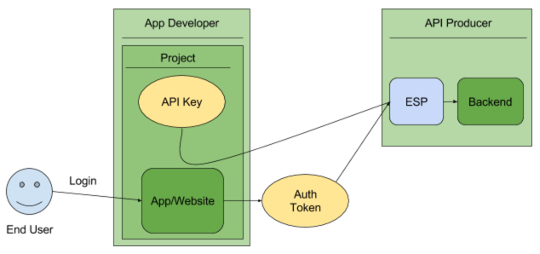
\includegraphics[width=0.6\textwidth]{api_keys_overview.png}
\end{center}
\end{figure}
\newpage
\section{Commissioning}
%
\hypertarget{commissioning}{}	
\blindtext[10]

\newpage

	
\end{document}
%opening 